%!TEX root = ../../Master.tex
\section{Analogue Navigation in Hospitals} % (fold 
\label{sec:anal_nav}
This section discusses existing analogue navigation platforms in order to draw experience from these. Strengths and weaknesses are analysed, providing a solid base for advancements in hospital navigation to be made in this paper. The main source of information for this section is a trip to Sygehus Nord in Aalborg. The reason for visiting Sygehus Nord was to get an idea of how navigating a hospital is. By experiencing the problem in real life, the need for an advancement in hospital navigation is further motivated.

Some figures in this section, were taken during the research at Sygehus Nord. Some of the assumptions made in \cref{sec:anal_nav} are based on the field research.

\subsection{Signs} \label{sub:sign}
Signs are usally used to mark key areas of a hospital. An example of a hospital sign would say \enquote{Main entrance} and \enquote{Ambulance entrance}\cite{signs_hospital,art_Osborne}.

Interior signs are typically affixed to walls, doors, windows or hang from the ceiling. These signs serve multiple purposes; they describe the location of the sign while other signs point to named areas and some will do both. If the hospital consists of multiple buildings, they can be numbered in order to navigate people to specific buildings. See \cref{fig:signs1,fig:signs2}.

Signs are good at guiding users because of their directional properties and their ability to provide relevant information at key positions.

On the other hand, signs can be hard to spot if the visitor is not familiar with hospitals. Sign can be obstructed visually by an overflow of signs or simply a big crowd. Another problem regarding signs, is that they imply the visitor to read. This is a problem if the reader cannot understand the language or is illiterate.\cite{signs_reading}. An overflow of information displayed on signs can confuse the user. This is due to the fact that signs are not personal.
An example; if the visitor is in building A and wants to visit a patient in building B, floor 6. It could become a challenge to set up enough signs to guide the visitor to the right building and floor, without flooding the other visitors with irrelevant information.

\begin{figure}
\centering
  \begin{minipage}{0.45\textwidth}
    \centering
    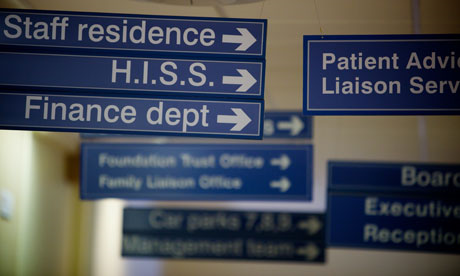
\includegraphics[width=\textwidth]{Alder-Hey-hospital-signs-007.png}
    \caption{Signs placed along a hallway. \cite{signs_hospital}} \label{fig:signs1}
  \end{minipage}
  \hfill
  \begin{minipage}{0.45\textwidth}
    \centering
    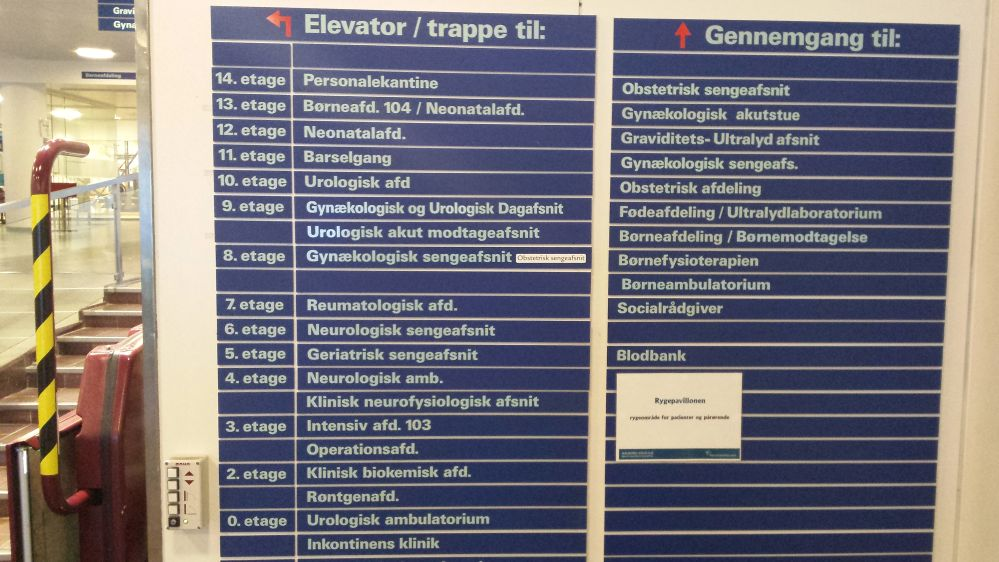
\includegraphics[width=\textwidth]{tavle.jpg}
    \caption{An overview sign of the different floors at Sygehus nord Aalborg} \label{fig:signs2}
  \end{minipage}
  \end{figure}

\subsection{Maps} \label{sub:map}
Analogue maps \cite{map} offer a top-down view of the hospital with all locations marked by text or colour \cite{art_Osborne}. See \cref{fig:map}. Maps can be affixed to walls or found in compact versions meant to be carried around. Stationary maps may have a red dot that marks the location of the map. By knowing the current position, the visitor's ability to navigate should improve as they will not have to scan their surroundings for recognizable objects identifying their position \cite{map_survey}. In case the building has multiple floors, the map will be split up into layers each depicting a floor in order to more easily represent a 3D structure.

Maps are able to efficiently show hot spots and quickly gain an overview on the location \cite{pros_analog_map}.

A common problem with maps is their greatly increased complexity when covering multiple floors \cite{map_confusing}. If the visitor is already inside the building, it can be difficult to figure out where they are corresponding to the map. If the visitors are in a hallway it can be difficult to distinguish it from the other hallways on the map.

  \begin{figure}[ht!]
  \centering
  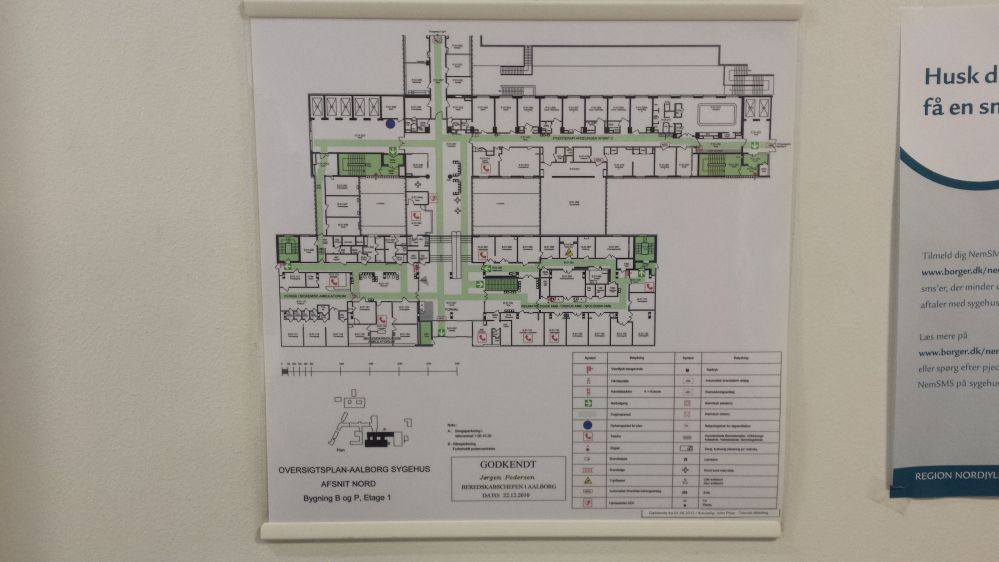
\includegraphics[width=90mm]{kortvaeg.jpg}
  \caption{A map on a wall at Sygehus nord Aalborg}
  \label{fig:map}
  \end{figure}

\subsection{Colour Coding}\label{sub:col}
Typically colour coding in hospitals are coloured lines painted on walls or floors. See \cref{fig:colour_floor}. They mark key routes to get to certain locations in the hospital. Usually a sign is describing the location the colours lead to. One line might say \enquote{recovery} and if followed, will lead to the recovery department. Some departments also have an entire theme in a certain colour. In this way, it might become easier for some people to navigate the next time they visit the hospital, if they can remember the colours representing that department.
Places that use this method of navigation would seamlessly offer an easy way of letting the visitors navigate, because the information provided by the colours are very simple to understand.

A problem with colour coding is that it is very static. If for example some rooms switches their function the stripes on the wall have to be repainted which will be a lot of work. If there are stripes leading to all the different departments, the information could potentially clutch up and become confusing. This method shares a downside with signs, as people with reading disorders or colour-blind have trouble with this navigation type

\begin{figure}[htb]
  \begin{center} 
    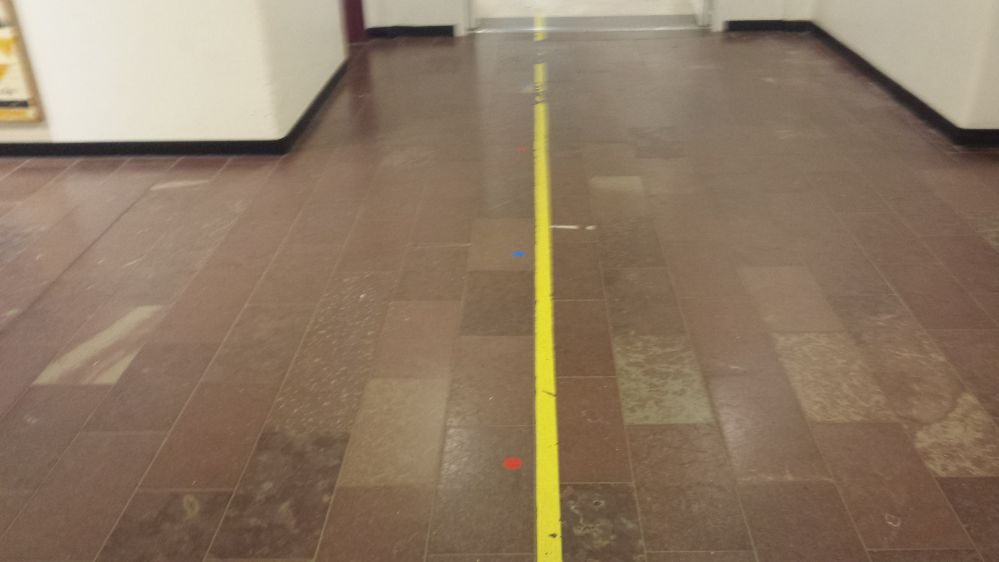
\includegraphics[width=0.5\textwidth]{stribe2.jpg}
  \end{center}
  \caption{Colour coding in use at Sygehus nord Aalborg}
  \label{fig:colour_floor}
\end{figure}

\subsection{Phone}\label{sub:pho}
Visitors are able to call the main number of the hospital and ask questions to a live operator. This can be done from any phone but there is no guarantee that a live operator is available. \cite{sign_ring}
 
The limitations regarding this navigation type are high as the informer is limited by only having voice as their tool. This can lead to  miscommunication. As said before, this type of navigation strictly depends on an assigned personal to answer the phone. If no one is at the phone, it becomes utterly useless.
If the service is frequently used, more than one employee might have to be assigned to the phone which would be a big resource hog.

\subsection{Human Interaction}\label{sub:human}
Visitors can ask hospital staff including receptionists regarding navigation around the hospital \cite{job}. This is much like the phone however human interaction has an advantage of being more precise. There will be less confusion as body language can be used in the answering of the question \cite{body_vs_phone}.

At \enquote{Sygehus Nord Aalborg} a receptionist booth is located at the main entrance. See \cref{fig:rec_booth}. If the visitor arrives at an entrance different from the main one, they might not know where the receptionist is if they need help. The information received from the receptions has to be memorized when the visitor ventures away from the desk. This means that directions could become hard to remember. To overcome this problem, receptionists could write a note but even so the text could be misinterpreted or in other ways mixed up.

  \begin{figure}[ht!]
    \centering
    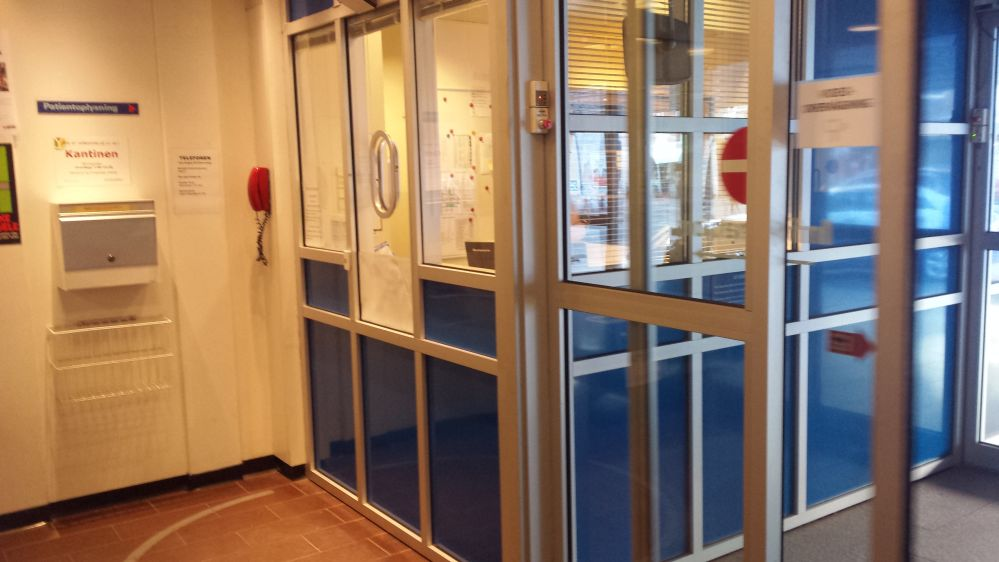
\includegraphics[width=90mm]{reception.jpg}
    \caption{A receptionist booth, seen at Sygehus nord Aalborg}
    \label{fig:rec_booth}
  \end{figure}

\subsection{Summary} % (fold)
  We found that in order to have a good navigation platform, the platform needs to be easy to interpret (\cref{sub:sign}), give a quick overview (\cref{sub:map}), be precise (\cref{sub:human}) and easy to understand (\cref{sub:col}). The design of our product has to avoid the weaknesses discovered in \cref{sec:anal_nav}. This means that the product must not display irrelevant information (\cref{sub:sign}), must deal with the representation of multiple floors in a non-confusing way (\cref{sub:map}), must deal with positioning without user interaction (\cref{sub:map}), and must be efficient in man hours to maintain (\cref{sub:pho}).